\section{Introduction to Ladder Logic} 
Figure~\ref{fig:ladderDiagram} depicts the ladder diagram for a button and a LED.  When the button is pressed the LED will illuminate, otherwise if the button is not pressed, then the LED will not illuminate. 

\begin{figure}[!htb]
\begin{center}
\tcbox[colframe=black,colback=white!30]{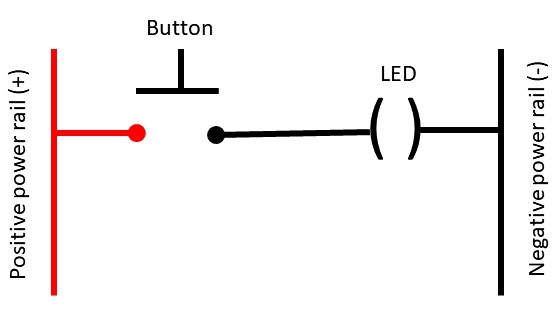
\includegraphics[scale=.8]{./images/LadderDiagram01.jpg}}
% 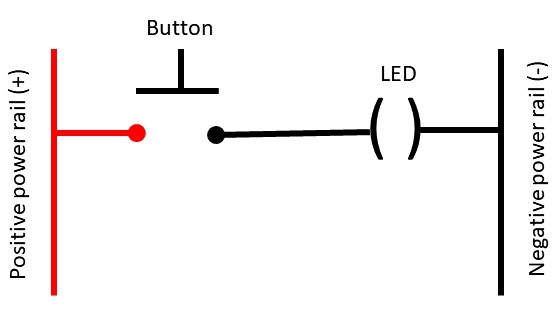
\includegraphics[width=0.5\textwidth]{./images/LadderDiagram01.jpg}
\end{center}
\caption{Ladder Diagram}
\label{fig:ladderDiagram}
\end{figure}

Notice the symbols of a Ladder Diagram (LD) are very similar to an electrical diagram. There are a few key differences between LD and electrical diagrams. (1) Ladder diagrams are read top to bottom from left to right, similar to how the pages in a book are read. (2) Order is very important for a LD, which resembles a ladder shape, of rungs of logic.

Starting from the top the LD is parsed and evaluated based on the current value of any inputs (example: contacts under the button). After the complete LD is read, the outputs are written (example: LED coil). If there is a discrepancy for the value of an output in the ladder logic, the last occurring rung determines the correct value for the output. 


\subsection{Relay Contacts}
A contact is a fundamental element of a ladder diagram. Figure~\ref{fig:relayContacts} depicts the different types of relay contacts. A contact is similar to a push button, and it has only two states: open or closed. A closed contact allows the the current flow to the next element. An open contact does not allow the current to flow to the next element.

\begin{figure}[!htb]
\begin{center}
\tcbox[colframe=black,colback=white!30]{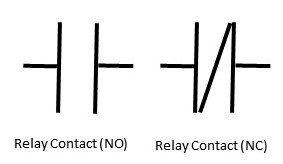
\includegraphics[scale=.75]{./images/LadderDiagram02.jpg}}
\end{center}
\caption[skip=-6pt]{Relay Contacts}
\label{fig:relayContacts}
\end{figure}

\subsubsection*{Relay Contact (Normally Open)}
A normally open relay contact referred to as examine when closed/on. If this contact is activated, usually by PLC input, then the current flows and the result is true.

\subsubsection*{Relay Contact (Normally Closed)}
A normally closed relay contact does not all the current to flow if the contact is closed. This contact behaves exactly opposite of the normally open relay contact. When activated, usually by PLC input, this normally closed relay contact will be false. 


\subsection{Coils}
A coil is a fundamental element of a ladder diagram. Figure~\ref{fig:coils} depicts the different types of relay contacts. A coil is similar to a relay contact in that is has two states. If the coil is activated it is said to be energized. If the coil is not activated it is said to be de-energized.

\begin{figure}[!htb]
\begin{center}
\tcbox[colframe=black,colback=white!30]{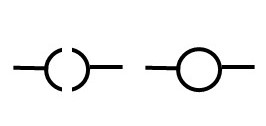
\includegraphics[scale=.80]{./images/LadderDiagram03.jpg}}
\end{center}
\caption[skip=-8pt]{Coils}
\label{fig:coils}
\end{figure}

\subsubsection*{The Open Coil}
Contacts are associated with inputs, coils are associated with outputs. If the series of instructions that precede the coil evaluate to true, the coil is energized. The activation of a coil can occur from writing to the PLC's I/O output device.

\subsubsection*{The Closed Coil}
The closed coil is similar to a normally closed rely contact. The coil closed coil is only energized when the series of instructions that precede the coil evaluate to false.

\subsection{PLC Logic and Scanning}
Similar to other programming languages, ladder diagrams can evaluate logical operations, including logical OR and logical AND. Figure~\ref{fig:logic} represents two common scenarios when evaluating a ladder diagram. 

\begin{figure}[!htb]
\begin{center}
\tcbox[colframe=black,colback=white!30]{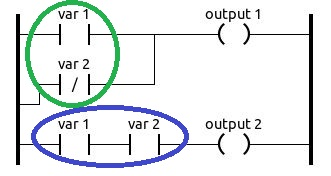
\includegraphics[scale=.8]{./images/LadderDiagram04.jpg}}
\end{center}
\caption[skip=-6pt]{PLC Logic and Scanning}
\label{fig:logic}
\end{figure}

\subsubsection*{Logical OR}
The green circle in Figure~\ref{fig:logic} represents a logical OR. The variable \textit{var1} can either be set or TRUE, or not set or FALSE. The variable \textit{var2} is a negated variable that can be set as TRUE; however because of the negation the output from \textit{var2} will be FALSE.  If \textit{var2} is not set or FALSE, then because of the negation of \textit{var2} the output will be TRUE. In the event that \textit{var1} is NOT set or FALSE and if negated \textit{var2} is not set the output of \textit{var2} will be TRUE causing the value for \textit{output1} will be energized or TRUE.

\subsubsection*{Logical AND}
The blue circle in Figure~\ref{fig:logic} represents a logical AND. In order for \textit{output2} to be energized or TRUE, then BOTH \textit{var1} and \textit{var2} MUST be activated or TRUE.

\subsubsection*{Scan Cycle}
The PLC Scan Cycle is the cyclic process by which PLCs operate. Recall there are three phases of a PLC Scan Cycle. In phase 1, all of inputs are read, and the value of each input is determined. In phase 2, the logic is processed. This logic relies on the value of each input. In phase 3, after the logic is processed, the outputs are determined and written. The output is determined by the last rung in the ladder to write to that output. 

\subsubsection*{Understanding Check \#1}
Using the logic from Figure~\ref{fig:logic} create a truth table for the possible inputs for \textit{var1} and \textit{var2} and the possible outputs for \textit{output1} and \textit{output2}. After you have completed the truth table answer the following questions.

\begin{adjustwidth}{.5cm}{0cm}
Truth Table for inputs and output of Figure~\ref{fig:logic} \\
    \begin{tabular}{|c|c|c|c|c|} 
    
    \hline
    \textit{var1} & \textit{var2} & neg \textit{var2} & \textit{output1} & \textit{output2}\\
    \hline
    \textit{False} & \textit{False} & & & \\
    \hline 
    \textit{False} & \textit{True} & & & \\
    \hline 
    \textit{True} & \textit{False} & & & \\
    \hline 
    \textit{True} & \textit{True} & & & \\
    \hline 
    \end{tabular}
    % \caption[skip=2pt]{Truth Table for inputs and output.}
    \label{table:understanindCheck1}
\end{adjustwidth}

\begin{enumerate}[noitemsep]
    \item What are the values for \textit{var1} and \textit{var2} for only \textit{output1} to be energized?
    \item What are the values for \textit{var1} and \textit{var2} for only \textit{output2} to be energized?
    \item What are the values for \textit{var1} and \textit{var2} for both \textit{output1} and \textit{output2} to be energized?
    \item What are the values for \textit{var1} and \textit{var2} for both \textit{output1} and \textit{output2} to NOT be energized?    
\end{enumerate}


\subsection{The Function Block}
Similar to other programming languages, ladder diagrams allow for relational operations.  Relational operations are provided through the use of function blocks. Figure~\ref{fig:logic} represents the different function blocks available for ladder diagrams. The behavior of each function block varies greatly and provides a great deal of functionality to Ladder Logic.

\begin{figure}[!htb]
\begin{center}
\tcbox[colframe=black,colback=white!30]{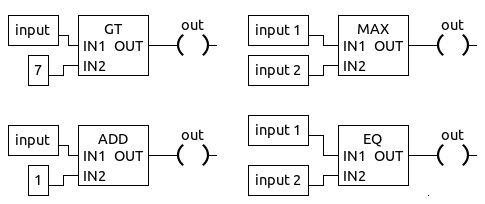
\includegraphics[scale=1]{./images/FunctionBlock01.jpg}}
\end{center}
\caption[skip=-6pt]{Function Blocks}
\label{fig:functionBlock}
\end{figure}

The Function blocks defined here (left to right, top to bottom) are: Greater Than (GT), Maximum (MAX), Addition (ADD), and Equality (EQ). Each of these function blocks accepts two inputs. The inputs can be a constant value such as a number, TRUE/FALSE, etc. or the inputs can be connected to the preceding instructions. The results of a function block can either be a boolean or numeric value, that is sent to the output labeled OUT.

\newpage
\subsubsection*{Understanding Check \#2}
Using the logic from Figure~\ref{fig:understanindCheck2}. Given all inputs labeled \textit{input2} and all outputs labeled \textit{output} are in the '0' or FALSE state answer the following questions.



\begin{figure}[!htb]
\begin{center}
\tcbox[colframe=black,colback=white!30]{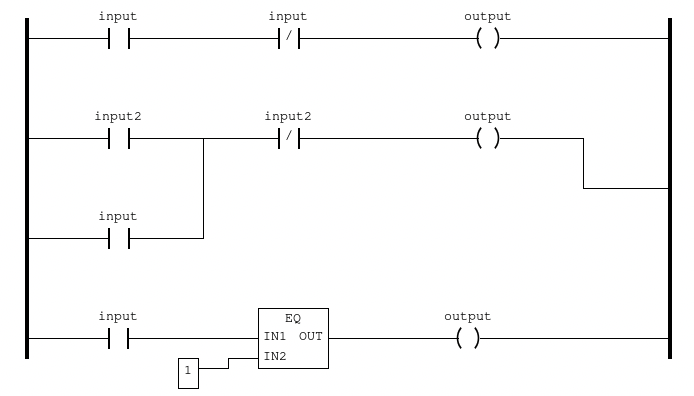
\includegraphics[width=.60\textwidth]{./images/LadderDiagram06.png}}
\end{center}
\caption{Ladder Diagram for Understanding Check \#2}
\label{fig:understanindCheck2}
\end{figure}

\begin{enumerate}[noitemsep]
    \item What will be the value of output after this ladder diagram is completed running?
    \item What are the values for \textit{input} and \textit{input2} are required for \textit{output} to be energized?
    \item Would the original output change if the function block IN2 also started at '0'?
\end{enumerate}

Similar to Understanding Check \#1, create a truth table for each of the inputs and outputs. Use this completed the truth table to justify your answers.
